\documentclass[journal,12pt,twocolumn]{IEEEtran}
\usepackage[cmex10]{amsmath}
\usepackage{amssymb}
\setlength{\parindent}{0pt}
\usepackage{array}
\usepackage{tikz, graphicx}
\usepackage{shadethm}
\usepackage{mathtools}
\usepackage{tcolorbox}


\title{Assignment 2}
\author{Danda Sai Pravallika  - CS20BTECH11013}

\begin{document}
\maketitle
Download all python codes from
\begin{tcolorbox}
https://github.com/spdanda/AI1103/blob/main/A
ssignment2/Assignment2.py
\end{tcolorbox}
and latex - tikz codes from 
\begin{tcolorbox}
https://github.com/spdanda/AI1103/blob/main/A
ssignment2/Assignment2.tex
\end{tcolorbox}
\large\textbf{Problem 5.31 :}\\
Two cards are drawn simultaneously (or successively without replacement) from a well-shuffled  pack  of  52  cards.  Find  the  mean, variance and standard deviation of the number of kings.\\
\textbf{Solution :}\\
Let X denote the no.of kings in a draw of 2 cards.
\begin{align}
\Longrightarrow\; \text{Pr(X=0)} &= \dfrac{48_{C_2}}{52_{C_2}}=\dfrac{188}{221} \\
\text{Pr(X=1)} &= \dfrac{4_{C_1}\text{ x }48_{C_1}}{52_{C_2}}=\dfrac{32}{221} \\ 
\text{Pr(X=2)}&=\dfrac{4_{C_2}}{52_{C_2}}= \dfrac{1}{221}\\ \nonumber
\end{align}
\vspace*{-2cm}
\begin{center}
\begin{tabular}{ | m{1.2cm} | m{1.5cm}| m{1.5cm} | m{1.5cm} | } 
\hline \vspace{2pt}

\large X     & \hspace{0.5cm}0                & \hspace{0.5cm}1               & \hspace{0.5cm}2             \\ \hline \vspace{6pt}
\large Pr(X) & \hspace{0.5cm}\(\frac{\textbf{188}}{\textbf{221}}\) & \hspace{0.5cm}\(\frac{\textbf{32}}{\textbf{221}}\) & \;\;\;\(\frac{\textbf{1}}{\textbf{221}}\)\\ 
\hline
\end{tabular}
\end{center}
\vspace{0.3cm}

Above is the probability distribution table of the no.of kings obtained when two cards are drawn simultaneously from a deck of 52 cards.
\begin{align}
\nonumber\text{Now, Mean of X}&= \text{E(X)} \\ \nonumber
               &=\sum_{k=0}^{2} \nonumber k\,\text{Pr(X=k)}\\\nonumber
               &= 0\times\frac{188}{221} + 1 \times\frac{32}{221} + 2 \times\frac{1}{221}\\
               &= \frac{34}{221} = 0.154\\\nonumber
\end{align}
\vspace*{-1.5cm}
\begin{align}
 \nonumber \text{Variance} &=\text{E}\,(\text{X}^2) - [\text{E}\,\text{X}]^2\\\nonumber
                  &= \sum_{k=0}^{2} k^2\text{Pr(X=k)} - \frac{34^2}{221^2}\\\nonumber
                  &= 1^2\times\frac{32}{221} + 2^2\times\frac{1}{221} - \frac{34^2}{221^2}\\\vspace{0.1cm}
                  &= \frac{6800}{48841} = 0.139\\\nonumber
\end{align}
\vspace*{-1.5cm}
\begin{align}
\nonumber\text{Standard Deviation }\sigma &= \sqrt{\text{Var(X)}}\\ \nonumber
&= \sqrt{0.139}\\ &= 0.373\\\nonumber
\end{align}

\newpage

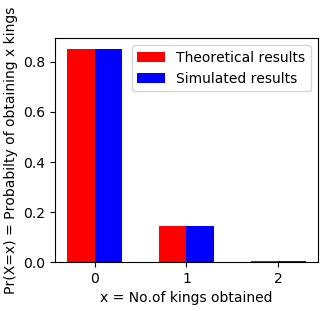
\includegraphics{Fig1.png}

 Above is the bar graph showing both the simulated and the theoretical results. Both represent almost the same values. 


\end{document}